% Set up page specifications and import packages
\documentclass[11pt]{amsart}
\usepackage[margin=.5in]{geometry}          
\usepackage{graphicx}
\usepackage{amsthm, amsmath, amssymb}
\usepackage{setspace}
\setlength{\parindent}{0em}
\usepackage{epsfig,bm,color}
\usepackage{mathtools}

\DeclarePairedDelimiter{\ceil}{\lceil}{\rceil}

% Define commonly used commands with a shortcut
\newcommand{\Zpx}{\mathbb{Z}_p[x]}
\newcommand{\Z}{\mathbb{Z}}
\newcommand{\Q}{\mathbb{Q}}
\newcommand{\C}{\mathbb{C}}
\newcommand{\R}{\mathbb{R}}
\newcommand{\e}{\epsilon}
\newcommand{\adj}{\rightarrow}
\newcommand{\tab}{\hspace*{.75cm}}
\newcommand{\setTo}{\leftarrow}
\newcommand{\ul}{\underline}
\newcommand{\kap}{\kappa}

% Define document tittle and author
\title{MA4710 Project 1}
\author{Daniel Henderson}

% Begin document and make tittle
\begin{document}
\maketitle

{\bf Introduction}\\

This report asses the validity of the assumptions of the regression model defined by,
$$ Y \cong \beta_0 + \beta_1X_1 + \beta_2 X_2 + \beta_3 X_3 + \beta_4 X_4 + \beta_5 X_5$$
where,\\
\tab $Y$: Hardest V-Grade.\\
\tab $X_1$: Height (cm)\\
\tab $X_2$: Weight (kg)\\
\tab $X_3$: ApeIndex (cm)\\
\tab $X_4$: Years spent climbing\\
\tab $X_5$: Max pull-up reps\\

The source and cleaning of the data is described in my previous submission.
Note, the cleaning that I preformed certainly influenced my results - I nearly chopped the data set in half to $285$ observations.
As discussed, the deletion was biased towards members of the population who didn't know certain statistics.
They where partial observations so therefore they where removed.
Nonetheless, we carry on with a diagnostic analysis of the fitted model.

\newpage
{\bf Initial Data Exploration}\\

Below is the generated scatterplot matrix
\begin{center}
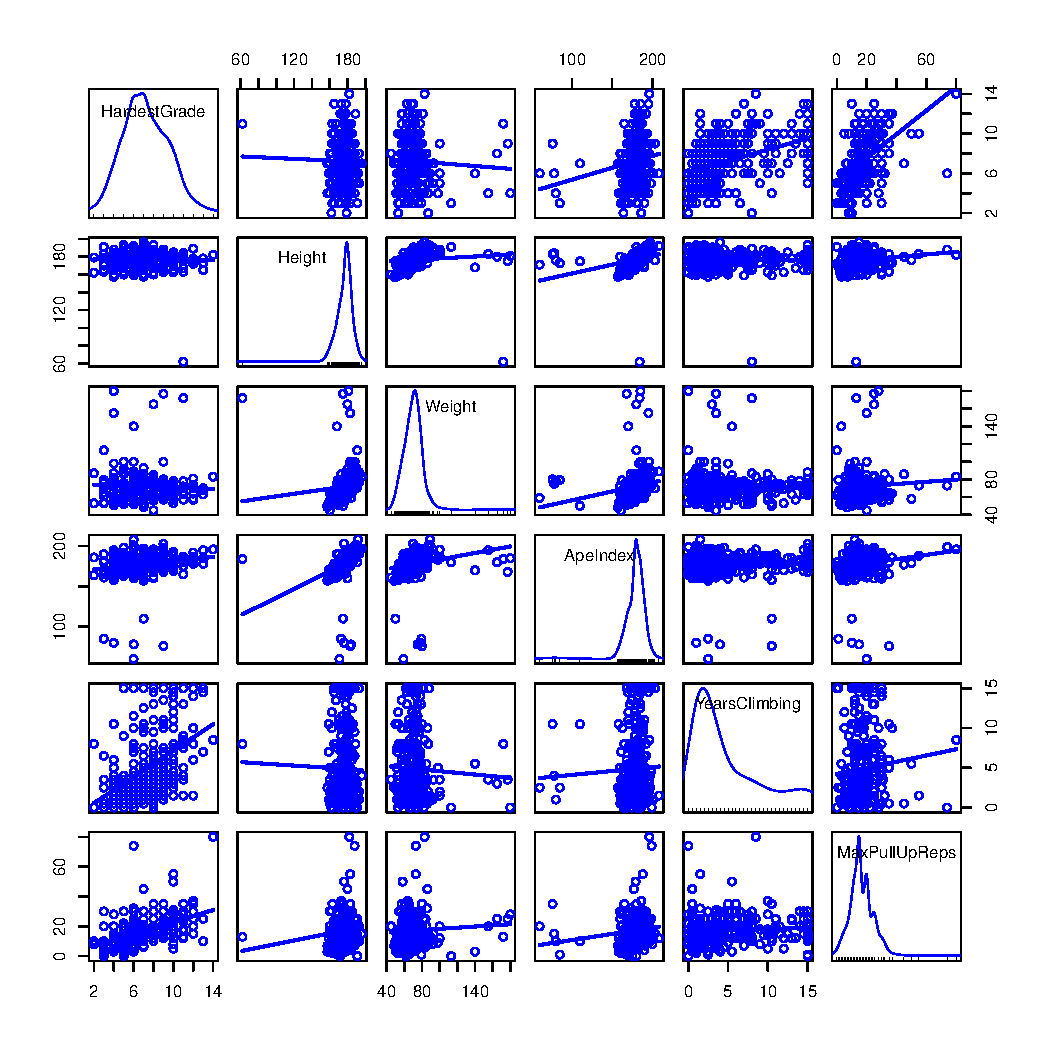
\includegraphics[width=0.65\textwidth]{1.pdf}
\end{center}

As shown above the response variable, HardestGrade, appears to be quite normal.
In fact when analyzing the diagonal elements in the graph above, HardestGrade is the only distribution that shows obvious signs of normality.
The $5$ other predictor variables all have a skewed distribution of some sort.
Another interesting observation is the possible simple linear relationship between HardestGrade and MaxPullUpReps.
There also may be a simple relationship between HardestGrade and YearsCliming.

\newpage
{\bf Assessment of Residual Normality Assumption}\\

Next we investigate the assumption that the residuals come from a population which is normally distributed.
The first graphical tool we use is the Q-Q plot of the standardized residuals which is shown below
\begin{center}
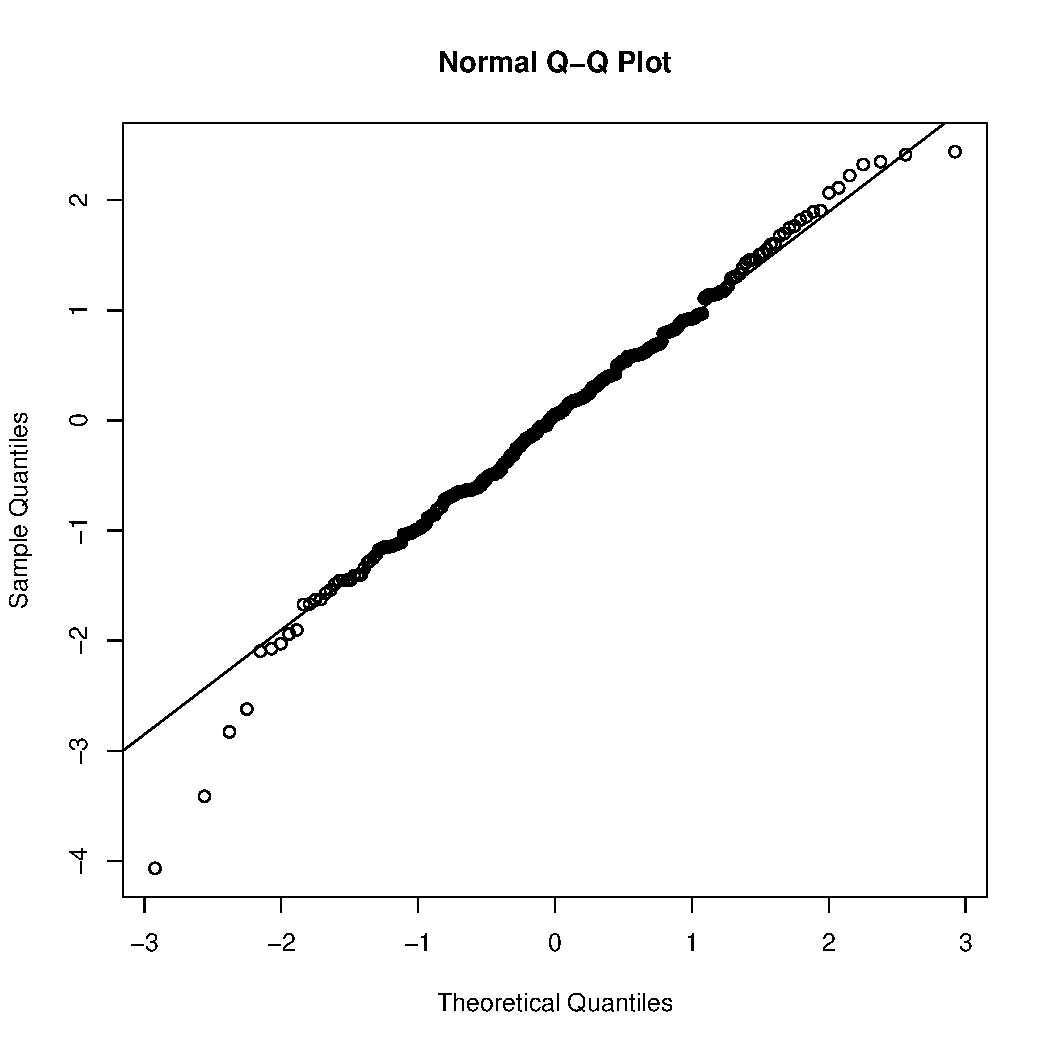
\includegraphics[width=0.65\textwidth]{2.pdf}
\end{center}

Looking at the left tail of the data, there is certainly reason to be concerned that our normality assumption is invalid.
The data should not deviate from the reference line as it does.\\

Additionally, the p-value of the Shapiro-Wilks test is $0.03573$, which is significant and we reject the null.
That is, we are roughly $96.5\%$ that the sample data did not come from a normally distributed population.
However, if we where perform this test at $2\%$ significance level, we would accept the null.
Since our data contains $285$ observations, the test may have detected trivial departures from the null hypothesis.
This has the effect of lowering our p-value. However, the Q-Q plot also showed signs of concern.
In conclusion, there is evidence to suggest that the normality assumption of our standardized residuals does not hold.


\newpage
{\bf Assessment of Linearity and Homoscedasticity Assumption}\\
Confirmation of the linearity assumption can be viewed as validation that we have chosen the correct model such that HardestGrade depends on the $5$ predictor variables in a linear fashion. We begin by looking at the plot of standardized residuals against each predictor variable and the fitted values of the model
\begin{center}
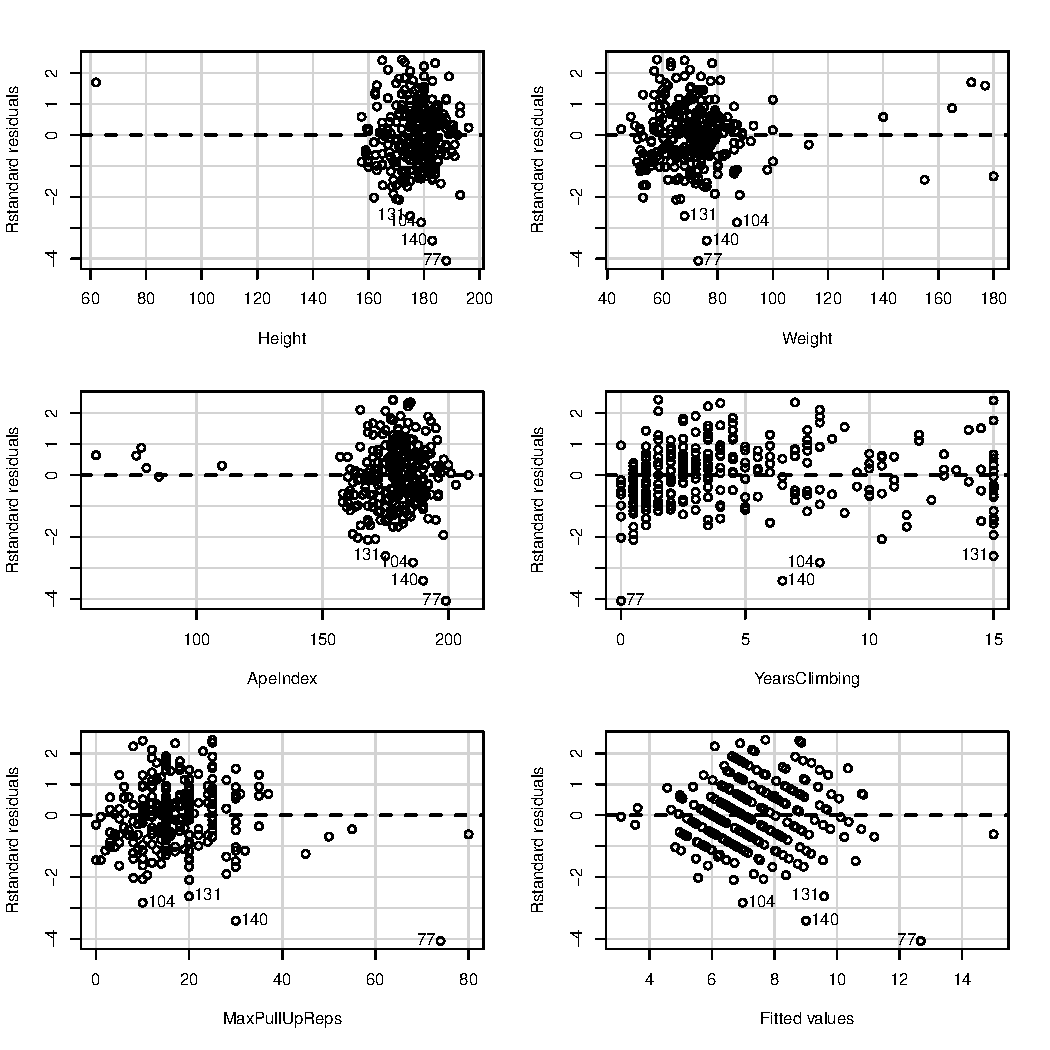
\includegraphics[width=0.65\textwidth]{3.pdf}
\end{center}
There is evidence to suggest that the linearity assumption of our model holds.
This is displayed by the lack of an obvious pattern in any of the above graphs.

\newpage
{\bf Assessment of Linearity and Homoscedasticity Assumption (Continued) }\\
However, upon further inspection on the previous page of the standardized residuals verse the fitted values plot, it appears that there may be a pattern there.
This could imply that our homoscedasticity assumption is under threat.
We can investigate this further by looking at the scale-location plot
\begin{center}
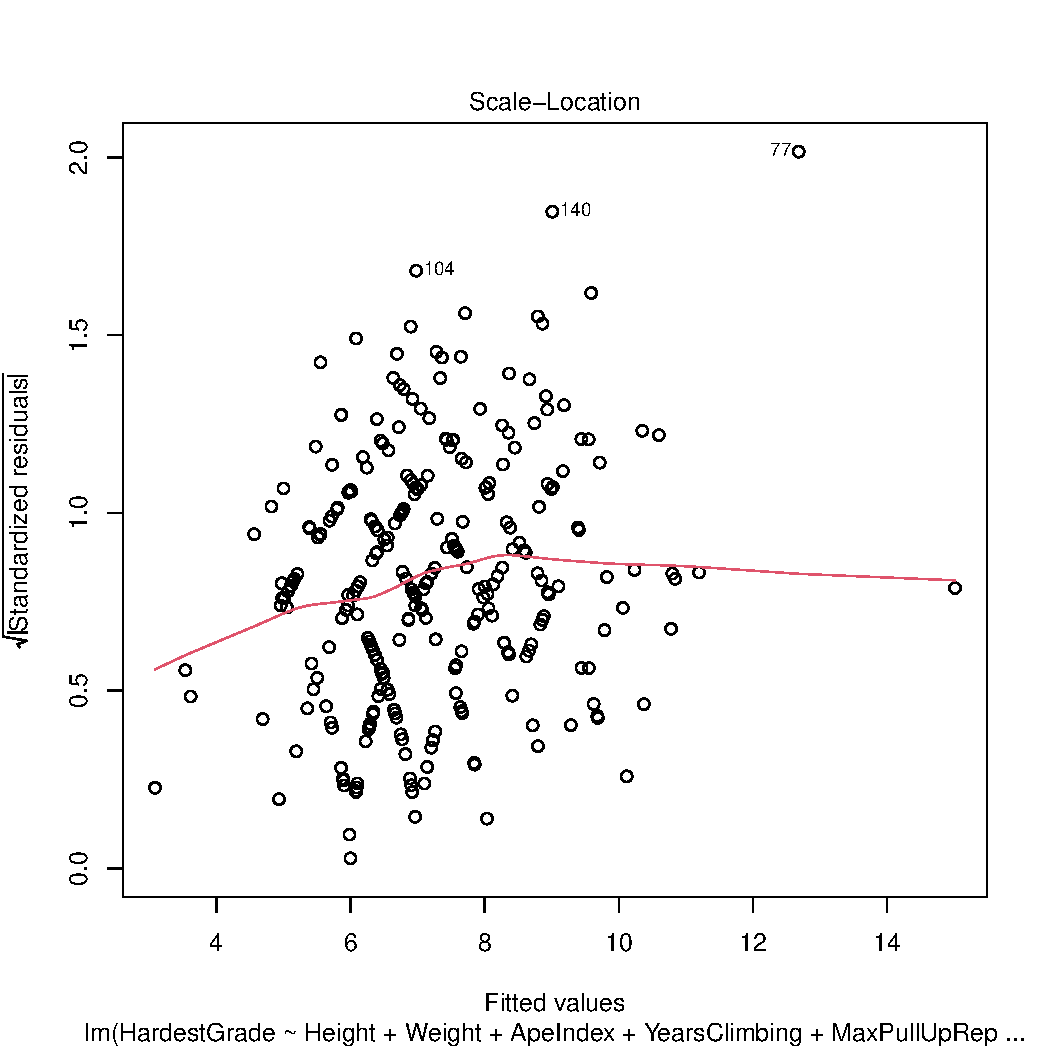
\includegraphics[width=0.65\textwidth]{4.pdf}
\end{center}
There is a slight increasing relationship in the graph which is evidence to reject the homoscedasticity assumption.
In conclusion, there is evidence to suggest that the residuals do not have a constant variance.

\newpage
{\bf One high-leverage and influential point}\\
The $22$-nd observation is a high-leverage point having a value of $0.63467327$.
This is more than $3$-times greater than the next highest leverage point.
This observation certainly needs to be investigated further.
Note, the average leverage value is approximately $0.017$ and they're $72$ observations that have a leverage higher than average.

Next observe the index plots of DFBETAS below
\begin{center}
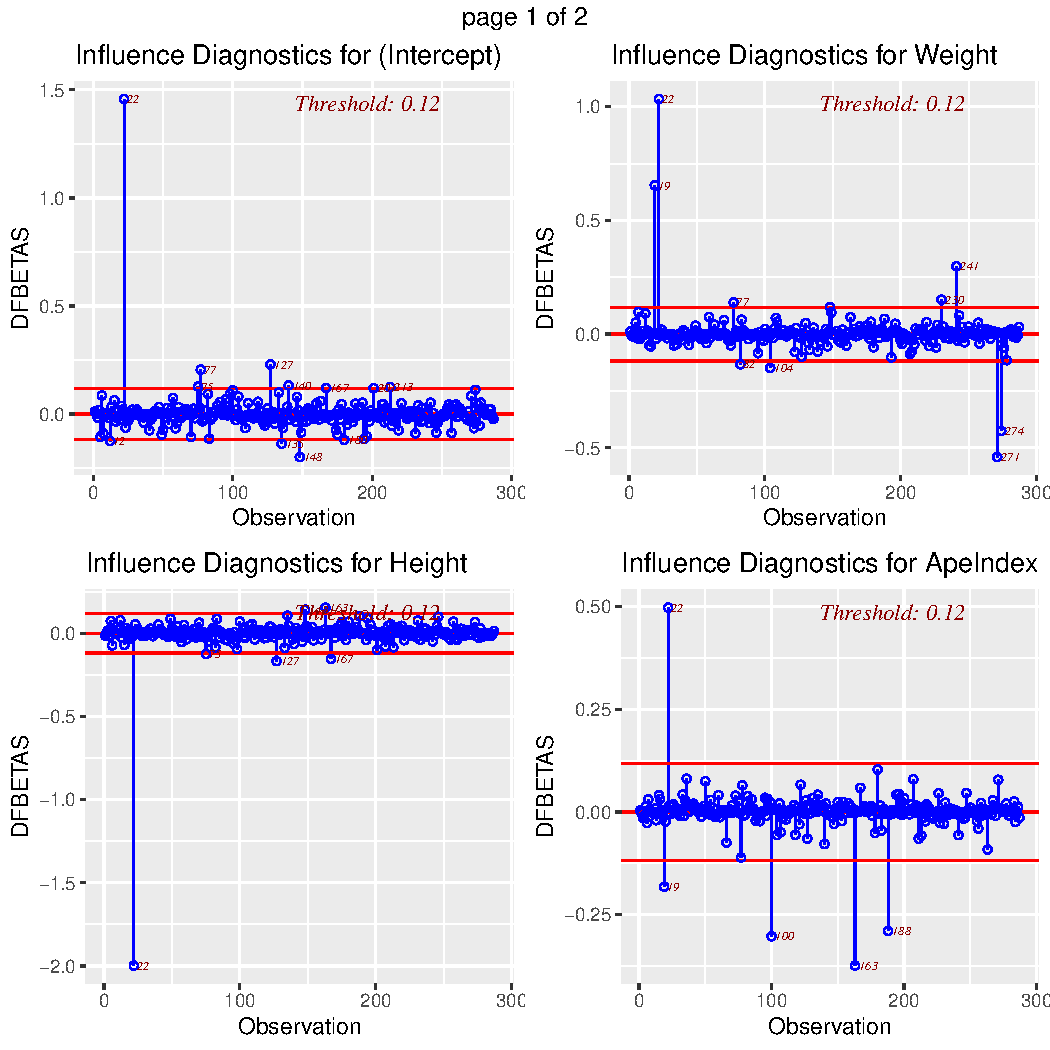
\includegraphics[width=0.5\textwidth]{8.pdf}
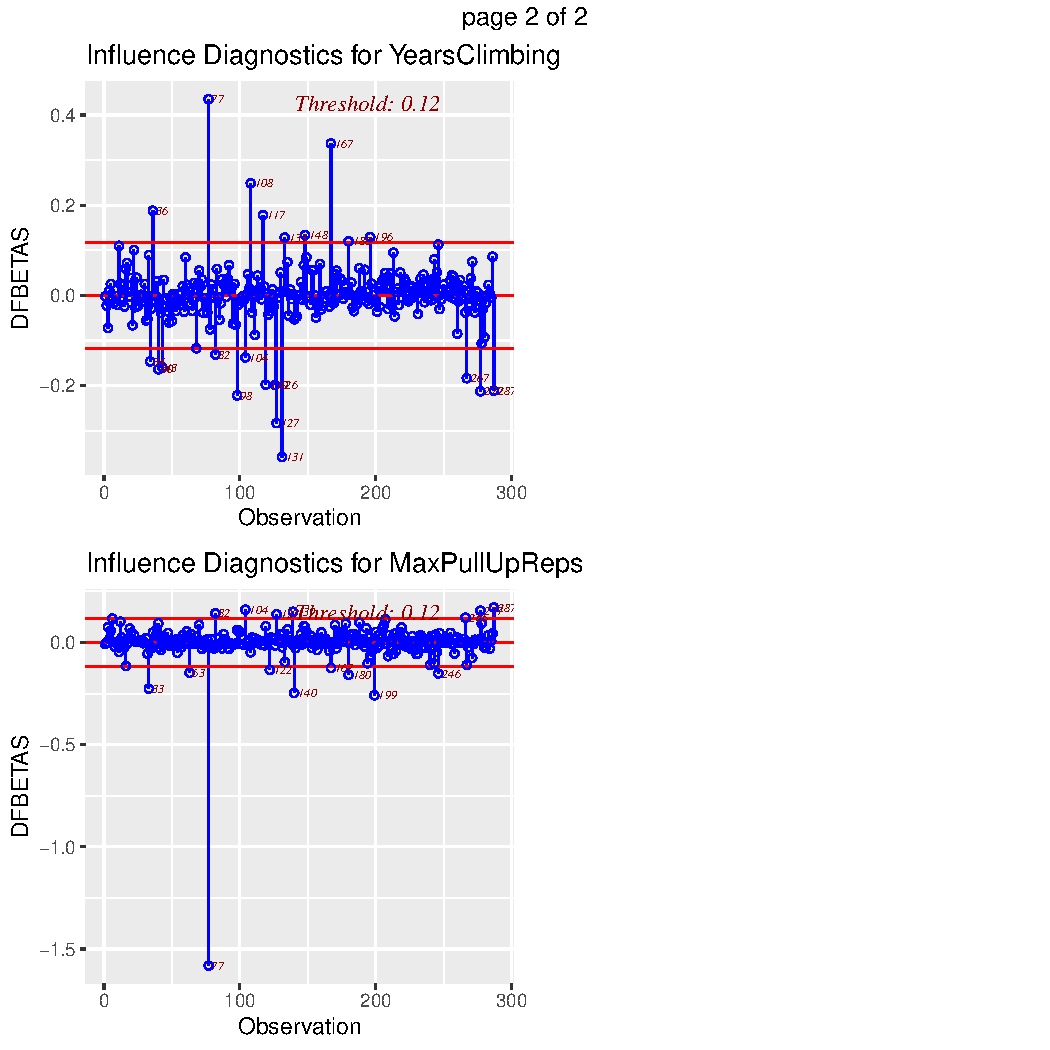
\includegraphics[width=0.5\textwidth]{9.pdf}
\end{center}
Note, you can also see that observation 22 occurs to have a significant impact on each regression coefficient.
Therefore, it is not only a high leverage point it is also a high influence point.

\newpage
{\bf Residual plus component Investigation}\\
\begin{center}
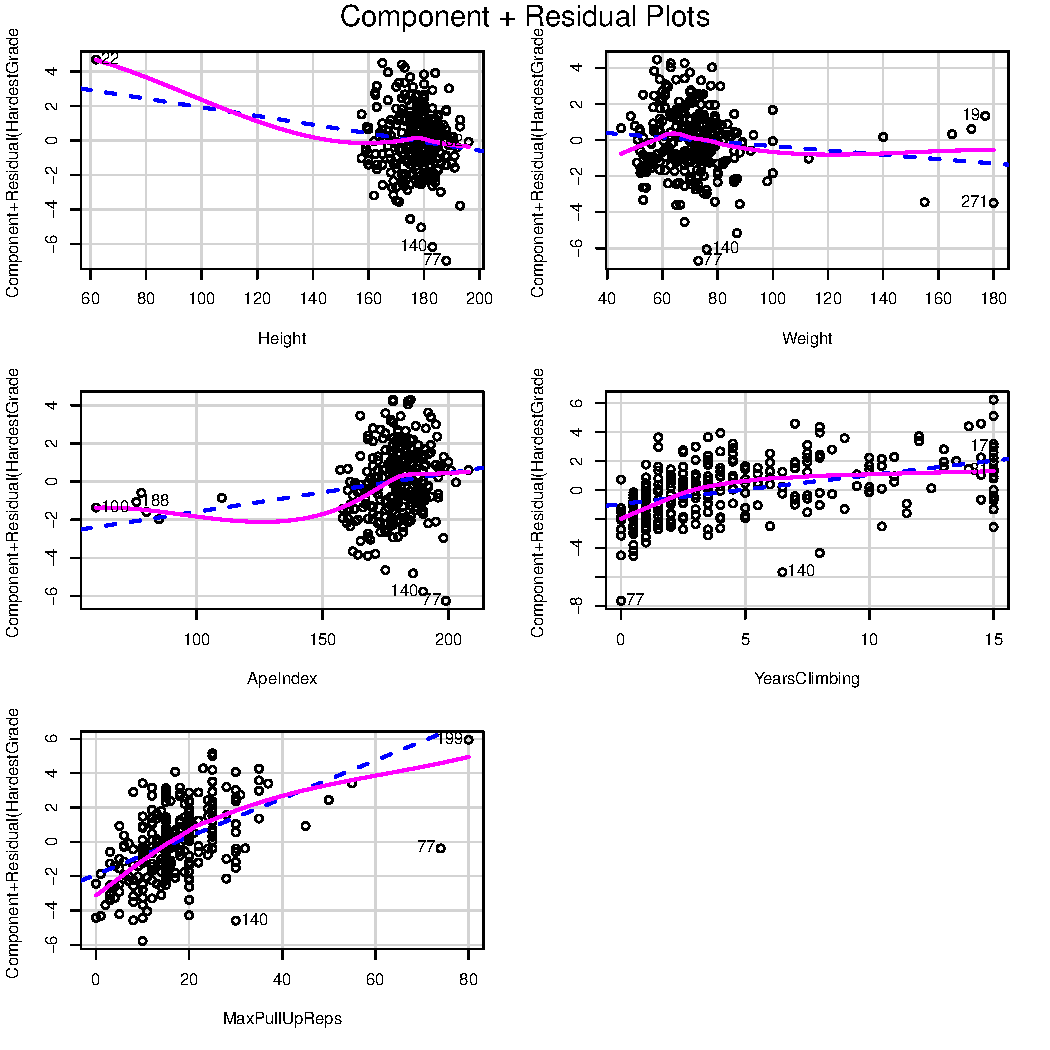
\includegraphics[width=0.65\textwidth]{10.pdf}
\end{center}

Looking at the first two plots associated with Weight and Height, there appears to be a quadratic relationship in the data so maybe we should take such an approach when adding them to our model. This makes a lot of sense. 
It is generally the average height and average weight (for a climber) that performs best.
Your performance would decrease if you deviate from the mean in either direction.\\

Similarly, looking at the plot associated with YearsClimbing, there appears to be a sutle logarithmic relationship.
This potentially means a transform is in order.
Note, this also makes sense because a simple model of learning any skill is best modeled by the logisitic ODE (which has a logarithmic solution). However, it appears a simple linear approximation will suffice. Since the slope is quite small, it doesn't add to much explanatory power to the model. Also, the p-value for the appropriate t-test is quite significant.\\

Lastly, looking at the ApeIndex and MaxPullUpReps plots, inside the data there is linear trend present.
This suggests that we are on the right track with these parameters and they add significant explanatory value to our response when added to the model. However, the observed significance of ApeIndex, isn't as low as I would like. This is likely due to the outliers shown on the left side of the plot.

\end{document}
